\setkomafont{title}{\Huge\rmfamily}
\addtokomafont{date}{\lining}


% \titlehead{%
%   
\includegraphics[height=1.2cm]{logos/tu.pdf}%
%   \begin{tikzpicture}[remember picture, overlay, shift=(current page.center)]
%     \node[anchor=center] at (0, 0) {%
%       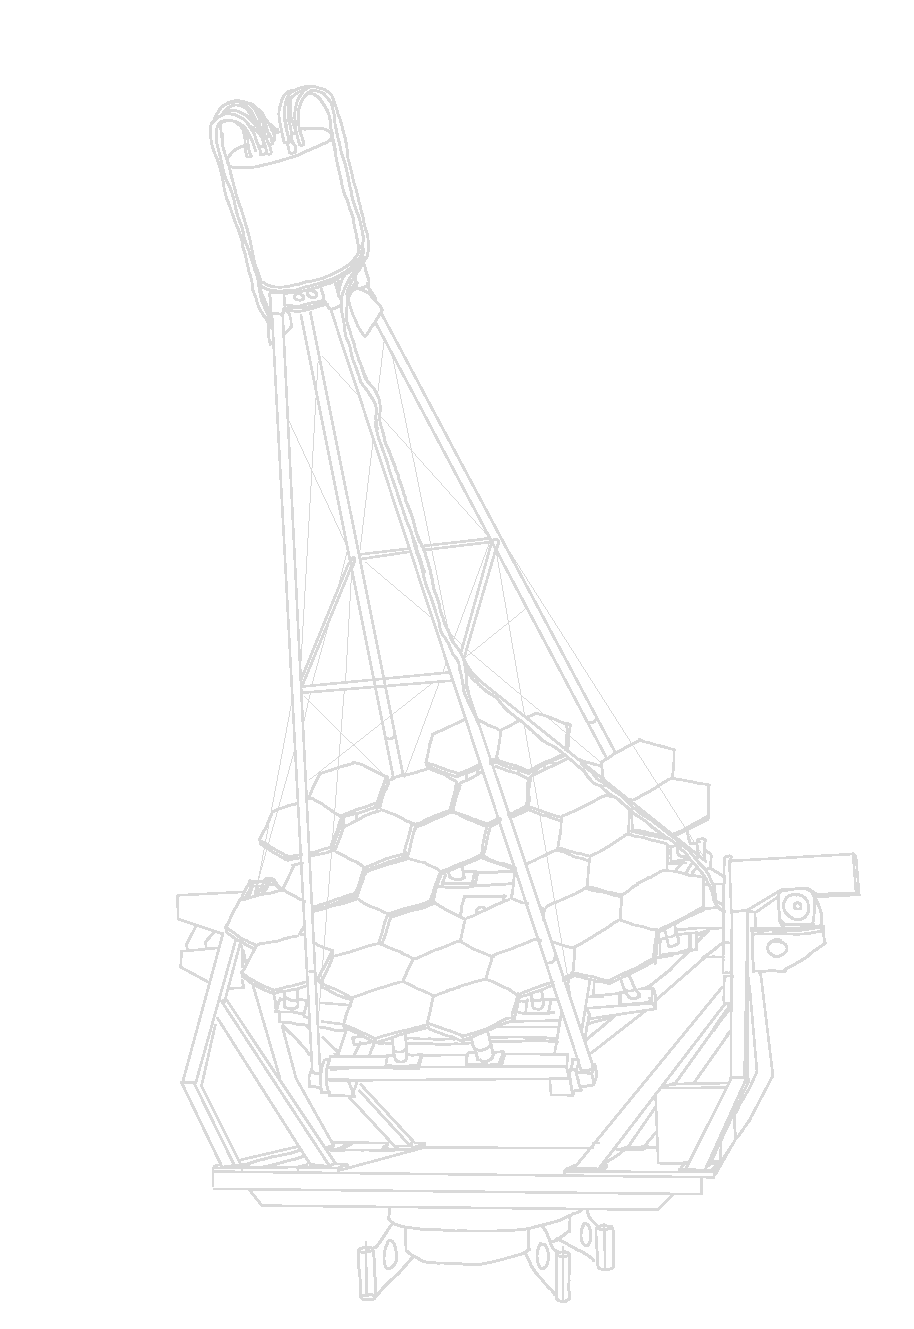
\includegraphics[width=\paperwidth-4cm]{images/fact_sketch.pdf}%
%     };
%   \end{tikzpicture}
% }
% \subject{%
%   Dissertation zur Erlangung des akademischen Grades \\
%   Doktor der Naturwissenschaften (Dr.~rer.~nat.)
% }
% \publishers{
%   Lehrstuhl für Experimentelle Physik 5\\
%   Fakultät Physik\\
%   Technische Universität Dortmund
% }
\makeatletter
\begin{titlepage}

  % background image
  \begin{tikzpicture}[remember picture, overlay, shift=(current page.center)]
    \node[anchor=center] at (0, 1cm) {%
      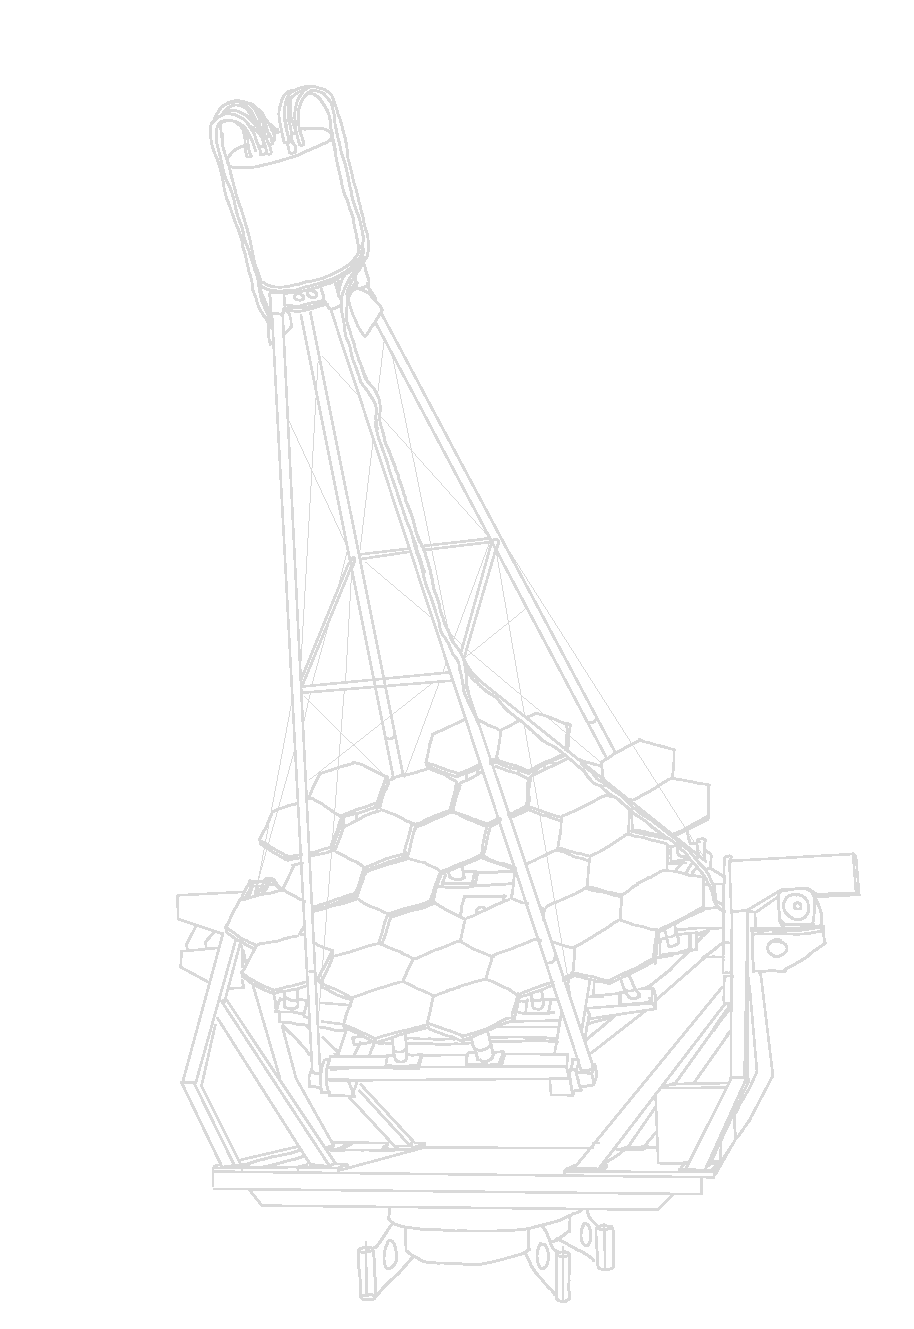
\includegraphics[width=\paperwidth-4cm]{images/fact_sketch.pdf}%
    };
  \end{tikzpicture}
  % TU logo
  \begin{tikzpicture}[remember picture, overlay, shift=(current page.north west)]
    \node[anchor=north west] at (\coverpageleftmargin, -\coverpagetopmargin) {%
    
\includegraphics[height=1.2cm]{logos/tu.pdf}%
  };
  \end{tikzpicture}

  \vspace*{5cm}
  \begin{center}
    {\usekomafont{title}\@title \\[0.5\baselineskip]}
    {\usekomafont{subtitle}\@subtitle\\[0.5\baselineskip]}
    {\usekomafont{author}\@author}\\
    {\usekomafont{date}\@date}\\

    \vspace{11cm}

    {\large%
      A document submitted in partial fulfillment of the requirements for the degree of \\
      \emph{Doctor rerum naturalium} \\
      at \\
      Fakultät Physik, Technische Universität Dortmund
    }

    \vfill
    {\large%
      Supervised by \\
      Prof.~Dr.~Dr.~Wolfgang~Rhode and Prof.~Dr.~Carsten~Westphal
    }%
  \end{center}
  % \endgroup
\end{titlepage}
\makeatother

\newpage
\thispagestyle{empty}
\vspace*{\fill}
\small\noindent%
This thesis is set in Libertinus (Serif, Sans and Math) and Fira Code,\\
typeset using \LaTeX{} with Lua\TeX{} from \TeX-Live 2020.\\
Title graphic by Sebastian A. Müller.
\newpage
